\documentclass{hw}

\title{Midterm Exam}
\author{MATH 168, Spring 2022}
\date{Due at 11:59pm, May 12th}

\begin{document}


\section*{MATH 168 Midterm Exam}


\subsection*{Exam Structure}

This is a 72-hour take-home midterm exam. 
It contains 8 problems. 
Many of these problems can be done independently of each other. 
\textbf{You do not need to do all the problems}. 
There is a total of 23 available points spread among the problems. 
Your score on the midterm can be at most 15. 
So, you can choose-your-own-adventure through the problems in order to aim for a total of 15 points. 

There are two main paths that I expect most of you will take. 
Both of them total 15 points. 
\begin{itemize}
    \item \textbf{Path 1: ``I like math more than coding.''} Problems 1, 2, 3, 4, 5, and 6. 
    \item \textbf{Path 2: ``I like coding more than math.''} Problems 1, 3, 5, 7, and 8. 
\end{itemize}
You're welcome to mix and match between these paths. 
However, it is likely a better use of your time to focus on doing one path really well than to put partial effort into problems from both paths. 

\subsection*{Grading}

This exam will be graded in a somewhat more traditional fashion: no re-attempts, but we will grant partial credit. 
To receive full credit on problems, you should: 
\begin{itemize}
    \item Carefully read all instructions. 
    \item Clearly explain your arguments and ideas, often using more words than mathematical symbols. 
    \item When coding, write concise code with helpful comments. 
\end{itemize}

\subsection*{``Extra Credit''}

For every 4 points you earn \textbf{beyond} 15, we'll give you a homework point. 
So, if you earn 19 points, you'll earn full credit on the midterm and 1 homework point. 
If you earn all 23 points, you'll get full credit on the midterm and 2 homework points. 


\section*{Permissible Resources}

You are welcome to consult any pre-existing resources, including Newman, lecture notes and videos from this course, and anything you can find on the internet. 
Please cite your sources when you use them, including a URL when applicable. 
You \textbf{may not} seek help from other human beings by discussing the exam or soliciting help on online forums such as Chegg or StackExchange. 

You are welcome to ask me questions of clarification. 
You can also ask me hints, although these will usually come with a ``point cost'' attached to them. 









\pagebreak






\subsection*{Mathematical Setup}

So far in MATH 168, we have seen several methods for \emph{ranking} nodes in graphs. 
These include betweenness centrality, PageRank, and Katz centrality. 
As you might expect, there are many others, and in this problem we will study one of them. 


The famous \emph{Cats Centrality} (CC, not to be confused with Katz centrality) is named for its primary historical application area of ranking famous cats on the internet. 
Like many other algorithms, CC ranks cats based on a series of pairwise comparisons. 
In standard deployments, users are shown pairs of cats, and asked to pick which one they like more. 
This process is repeated many times to form a \emph{directed network} of pairwise preferences. 
\Cref{fig:cat-rank} shows an example of such a directed network. 
Here, an arrow $i \rightarrow j$ means that a user preferred cat $j$ to cat $i$. 
Popular cats are cats with lots of incoming arrows and few outgoing arrows. 

\begin{figure}[h] 
    \centering
    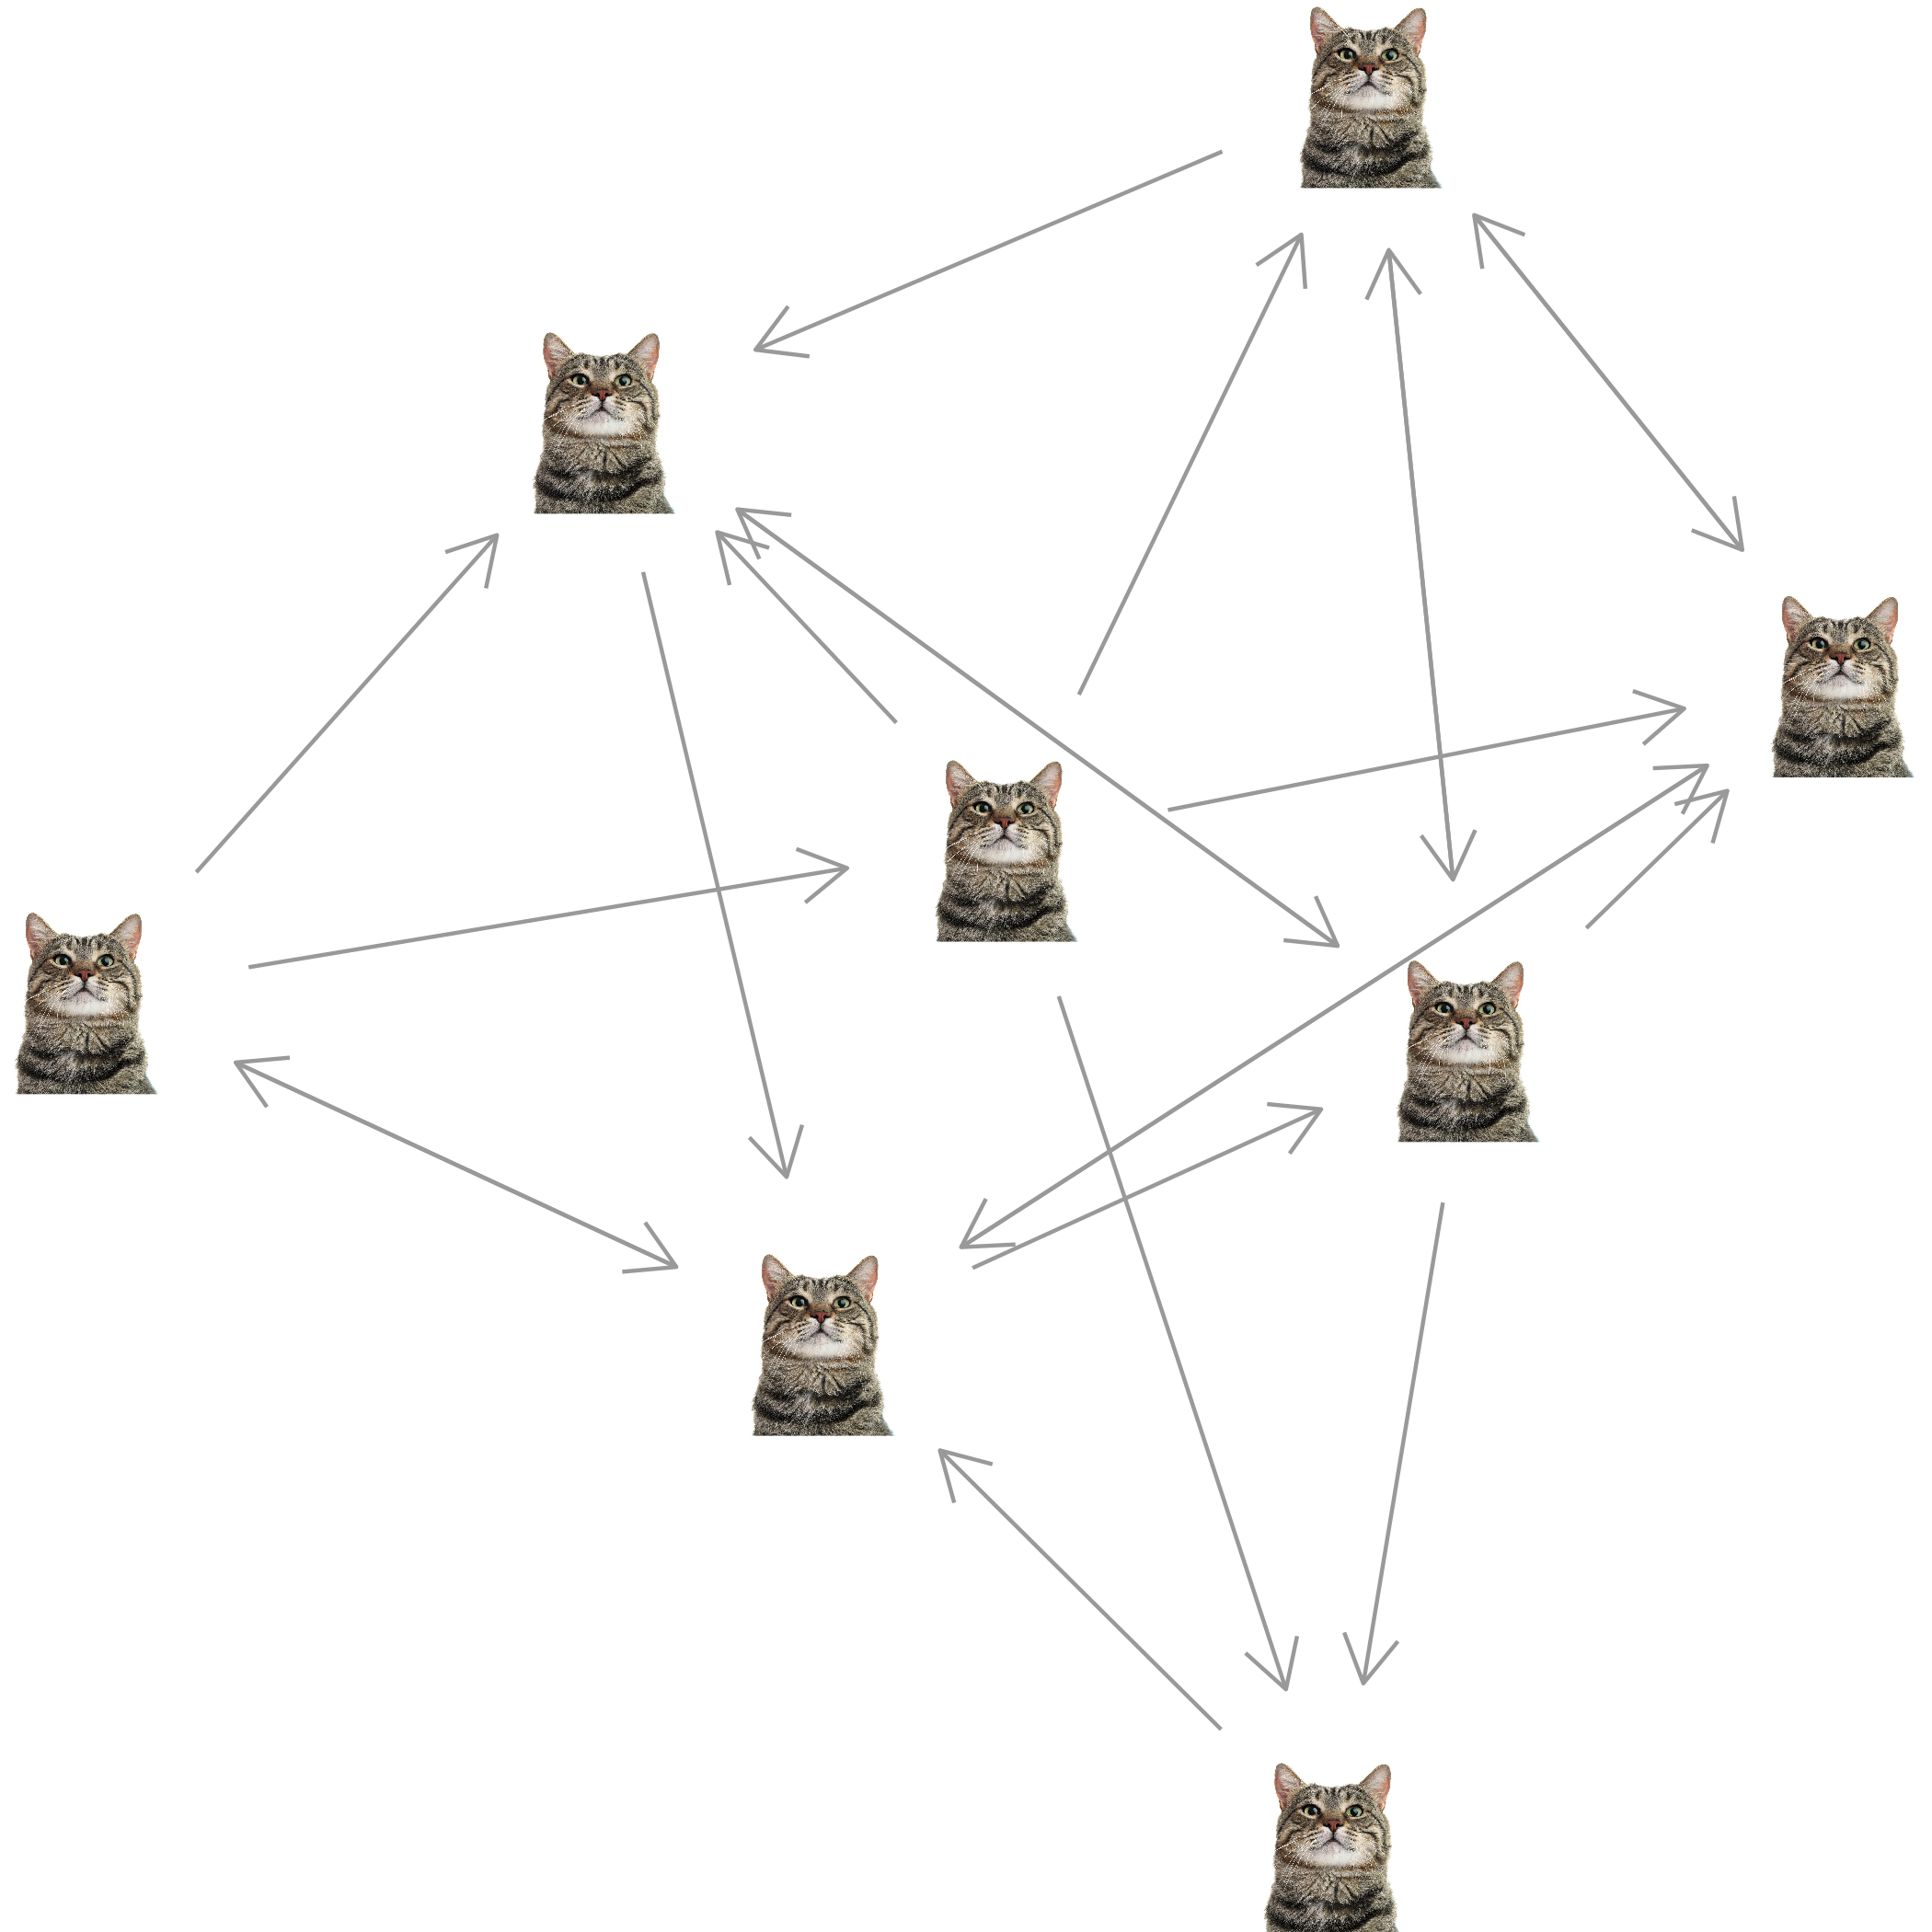
\includegraphics[width=.7\textwidth]{img/cat-rank.png}
    \caption{A directed network of pairwise preferences. 
    An arrow $i \rightarrow j$ means that a user preferred $j$ to $i$. 
    Links with arrows on both sides mean that one user preferred $i$ to $j$ and one user preferred $j$ to $i$.}   \label{fig:cat-rank}
\end{figure}


Consider a set of $n$ cats. 
Let $a_{ij}$ be the number of times that a user preferred cat $j$ to cat $i$. 
We can collect all these rankings in a \emph{directed adjacency matrix} $\mathbf{A} \in \mathbb{Z}_{+}^{n\times n}$. 
Note that $\mathbf{A}$ is not symmetric: in general, $a_{ij} \neq a_{ji}$.  
Additionally, we can have $a_{ij} > 1$ if multiple users preferred cat $j$ to cat $i$. 
We assume that there are no self-loops, i.e. $a_{ii} = 0$ for all $i$. 

Unlike methods we've seen based on random walks, counting paths, or eigenvector calculations, Cats Centrality is an \emph{optimization} model. 
The aim is to assign to each cat $i$ a rank $s_i \in \mathbb{R}$ such that a higher rank means an overall more preferable cat. 
The CC objective is a function that takes a vector of rankings $\mathbf{s}\in \mathbb{R}^n$ and returns a real number reflecting the quality of the ranking. 
Its mathematical structure is 
\begin{align}
    \mathrm{CC}(\mathbf{s}) = \sum_{i \in N}\sum_{j \in N}a_{ij}(s_j - s_i - 1)^2 + \lambda \sum_{i\in N}s_i^2\;, \label{eq:RCR}
\end{align} 
where $\lambda \geq 0$ is a scalar \emph{regularization parameter} that is usually chosen to be very small. 
The rankings are computed by solving the optimization problem 
\begin{align}
    \hat{\mathbf{s}} = \mathrm{argmin}_{\mathbf{s}\in \mathbb{R}^n} \mathrm{CC}(\mathbf{s})\;. 
\end{align}
That is, the ranking vector $\hat{\mathbf{s}}$ is a vector that makes the objective function as small as possible. 

\problem{(2 points, Path 1 and Path 2)} 

Assume in this problem that $\lambda = 0$ (this is called \emph{unregularized Cats Centrality}). Consider the simple network of pairwise comparisons shown in \Cref{fig:path}. 
Each arrow corresponds to a single pairwise comparison. 
Find a ranking vector $\mathbf{s}\in \mathbb{R}^6$ that achieves $\mathrm{CC}(\mathbf{s}) = 0$, and explain why this is the smallest possible value that the CC objective function can achieve.  
Then, find a \textbf{second} ranking vector $\mathbf{s}'$ that also achieves $\mathrm{CC}(\mathbf{s}') = 0$. 

\begin{figure}[h]
    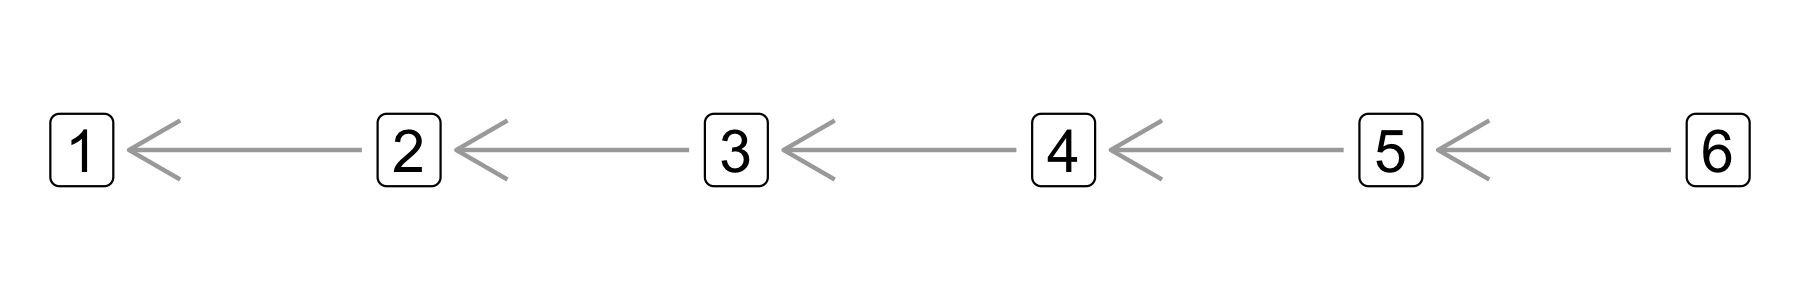
\includegraphics[width=\textwidth]{img/path.png}
    \caption{A path network of pairwise comparisons.}\label{fig:path}
\end{figure}

\begin{hint}
    Remember, an arrow $i \rightarrow j$ means that $j$ is preferred to $i$. 
    So, in your solution, the node with the highest score should be node $1$. 
\end{hint}

\problem{(5 points, Path 1)} 

Show by direct calculation that the equation $\nabla \mathrm{CC}(\mathbf{s}) = 0$, with the $\mathrm{CC}$ objective function given by \eqref{eq:RCR}, is equivalent to the following linear system: 
\begin{align}
    \left[\mathbf{K}^\mathrm{out} + \mathbf{K}^{\mathrm{in}} - (\mathbf{A} + \mathbf{A}^T) + \lambda \mathbb{I}\right]\mathbf{s} = [\mathbf{K}^{\mathrm{in}} - \mathbf{K}^\mathrm{out}]\mathbf{1}\;.  \label{eq:linear-system}
\end{align}
Here, 
\begin{itemize}
    \item $\mathbf{K}^{\mathrm{in}}$ is a diagonal matrix. 
    Its diagonal entries $k_i^{\mathrm{in}}$ count the number of times node $i$ was preferred in a pairwise comparison, also called the \emph{in-degree}. 
    The in-degree can be computed as $k_i^{\mathrm{in}} = \sum_{j \in N}a_{ji}$. 
    \item Similarly, $\mathbf{K}^{\mathrm{out}}$ is a diagonal matrix. 
    Its diagonal entries $k_i^{\mathrm{out}}$ count the number of times node $i$ was \textbf{not} preferred in a pairwise comparison, also called the \emph{out-degree}. 
    The out-degree be computed as $k_i^{\mathrm{out}} = \sum_{j \in N}a_{ij}$. 
    \item $\mathbb{I}$ is the matrix identity. 
    \item $\mathbf{1} = (1,1,\ldots,1)^T$ is the vector of $n$ copies of the number $1$. 
\end{itemize}

\begin{note}
    This calculation shows that solving \eqref{eq:linear-system} for $\mathbf{s}$ will yield a critical point of the Cats Centrality objective function \eqref{eq:RCR}. 
    It's true that, if $\lambda > 0$, this critical point is in fact the \emph{global minimum}. 
    Demonstrating this is the subject of Problem 6. 
\end{note}

\begin{hint}
    When performing this calculation, you might find it useful to remember that $a_{ii} = 0$ for all $i \in N$. 
\end{hint}

\problem{(3 points, Path 1 and Path 2)}

\emph{Although this problem involves an equation shown in Problem 2, you don't need to complete Problem 2 to complete this problem.}

Assume that $\lambda > 0$. 
Suppose that $\mathbf{A} = \mathbf{A}^T$. 
This scenario corresponds to the case that, for every pair $(i,j)$, cat $j$ is preferred to cat $i$ exactly as often as cat $i$ is preferred to cat $j$. 
Using \eqref{eq:linear-system}, prove that $\mathbf{s} = \mathbf{0}$. 
That is, all cats have the same Cats Centrality in this case. 

\begin{hint}
    Recall that, in order to prove that $\mathbf{x} = \mathbf{0}$ is the unique solution of the linear system $\mathbf{M}\mathbf{x} = \mathbf{b}$, it is necessary to prove something about \emph{both} $\mathbf{M}$ and $\mathbf{b}$. 
\end{hint}


\problem{(2 points, Path 1)}

Let $\mathbf{s}(\lambda)$ be the solution of \eqref{eq:linear-system} for fixed $\lambda$. 
Consider the vector
\begin{align}
    \mathbf{t} \triangleq \lim_{\lambda \rightarrow \infty} \lambda\mathbf{s}(\lambda)\;. 
\end{align}
Give a formula for $\mathbf{t}$ in terms of the vectors and matrices appearing in \eqref{eq:linear-system}.
You should explain how you came to your answer, but you do not need to give a formal proof.  

\begin{note}
    Intuitively, this result shows that choosing $\lambda$ too large makes the Cats Centrality kind of boring. 
    This is the reason that we usually choose small values of $\lambda$. 
\end{note}


\problem{(2 points, Path 1 and Path 2)}

Consider the unregularized Cats Centrality, which corresponds to $\lambda = 0$. 
Prove that, if $\mathbf{s}$ is a solution of \eqref{eq:linear-system} in this case, then so is $\mathbf{s} + \alpha \mathbf{1}$ for any $\alpha$. 
Here, $\mathbf{1}$ is the vector containing all ones. 

\begin{note}
    This property is often called \emph{translation invariance}.
    In the context of data analysis, it's usually considered to be a nuisance, since it means that there isn't a single ``right'' answer. 
    The purpose of setting $\lambda > 0$ in practice is to remove translation invariance. 
\end{note}

\problem{(1 point, Path 1)}

Prove using any method that the Hessian (matrix of second derivatives) of the Cats Centrality objective function $\mathrm{CC}$ with respect to the entries of $\mathbf{s}$ is positive-definite provided that $\lambda > 0$. 

\begin{note}
    It follows from this fact that the solution to \eqref{eq:linear-system} is in fact the unique global minimizer of the the the Cats Centrality objective \eqref{eq:RCR}. 
    So, if $\lambda > 0$, there is a \emph{unique} set of rankings returned by the Cats Centrality algorithm.   
\end{note}

\begin{hint}
    Can you relate the matrix $\mathbf{K}^\mathrm{out} + \mathbf{K}^{\mathrm{in}} - (\mathbf{A} + \mathbf{A}^T)$ to a matrix we've seen before? 
\end{hint}











\problem{(5 points, Path 2)}

\emph{In this problem you need to read and understand the linear system in \eqref{eq:linear-system}. However, you can complete this problem without completing Problem 2.}

In Python or your favorite programming language, write a function called \texttt{cats\_centrality} that implements the regularized Cats Centrality of a directed network. 
Your function should accept two arguments: a directed graph of pairwise comparisons and the regularization parameter $\lambda > 0$. 
Here's what to do: 
\begin{itemize}
    \item First, write a helper function called \texttt{compute\_matrices} that computes and returns the matrices that appear in \eqref{eq:linear-system}. 
    \item In your \texttt{cats\_centrality} function, first call \texttt{compute\_matrices} to get all the matrices you need to define the linear system \eqref{eq:linear-system}. 
    Then, use a standard function for solving linear systems to find the solution $\mathbf{s}$. 
    \item Return the solution $\mathbf{s}$. 
\end{itemize}
Include comments throughout your code to help us understand what you're doing. 
Additionally, please spend some effort to make your code as simple and brief as reasonably possible. 
For full credit, please ensure that \texttt{compute\_matrices} is \textbf{under 15 lines of code} (excluding comments), and that \texttt{cats\_centrality} is \textbf{under 5 lines}. 
\textbf{Each line should be under 80 characters long}. 
In fact, it's possible to implement both solutions in many fewer lines than that, especially if you are comfortable with Numpy array programming or its equivalents. 
My own solutions were 5 and 2 lines, respectively. 

For this problem, all you need to do is submit carefully documented code -- no outputs necessary. 

\begin{hint}
    In Python with NetworkX and Numpy, the following code will compute the adjacency matrix of a directed graph \texttt{G} as a 2D Numpy array: 
    \begin{verbatim}
        A = nx.to_numpy_array()
    \end{verbatim}
\end{hint}

\begin{hint}
    If you are less comfortable constructing matrices, vectors, and linear systems in Python, you might benefit from \href{https://nbviewer.org/github/PhilChodrow/PIC16B/blob/master/lectures/math/linear-algebra-I.ipynb}{these lecture notes}. 
    If you are less comfortable with creating and manipulating arrays in general, you might benefit from \href{https://jakevdp.github.io/PythonDataScienceHandbook/02.00-introduction-to-numpy.html}{this book chapter}. 
\end{hint}



\problem{(3 points, Path 2)}

The data at the URL below contains a list of edges for a network of directed comparisons. 
\begin{verbatim}
    https://raw.githubusercontent.com/PhilChodrow/
    intro-networks/main/data/sample-data.csv 
\end{verbatim}
It has a \texttt{source} column and a \texttt{target} column. 
In each case, the \texttt{target} column is preferred to the \texttt{source} column. 

Read this data into your software of choice. 
Then, compute the Cats Centrality for each node in the data, using your implementation from the previous problem. 
You can use the regularization parameter $\lambda = 0.1$. 
Then, 

\begin{itemize}
    \item Create a network visualization in which the size or color of each node corresponds to its Cats Centrality. 
    Please make sure that edges in your visualization are appropriately labelled with arrows to indicate the direction of comparison. 
    \item Submit the image in the accompanying data directory corresponding to the node with the highest Cats Centrality. 
    For example, if node $0$ is the highest-ranked, please show the image \texttt{cats/0-maru.jpeg} in your submission.   
\end{itemize}

\begin{hint}
    If you are working in Python with NetworkX, the following code will correctly construct a directed network from the data. 
    \begin{verbatim}
        url = "https://raw.githubusercontent.com/PhilChodrow/
        intro-networks/main/data/sample-data.csv"
        df = pd.read_csv(url)
        G = nx.from_pandas_edgelist(df, create_using = nx.DiGraph)
    \end{verbatim}
    If you run into problems related to accessing the data directly from online, you can instead download the data and read it in from your local filesystem. 
\end{hint}









\pagebreak 

\begin{figure}[h]
    
\includegraphics[width=\textwidth]{img/unbutterable.jpeg}
    \caption{The current \#BestCat on the entire internet, as determined by Cats Centrality. \href{https://twitter.com/JortsTheCat/status/1509705795486724098?s=20&t=k_XvXEFp33ImE4xRyNAfcA}{Image source}.}
\end{figure}




\end{document}